\documentclass[a4paper,11pt]{exam}

\usepackage[T1]{fontenc}
\usepackage[top=2cm, bottom=2cm, left=2.5cm, right=2.5cm]{geometry}
\usepackage{amsmath,amssymb}
\usepackage{amsthm}
\usepackage{hyperref}
\usepackage{bm} % bold greek
\usepackage{tcolorbox}
\usepackage{xcolor}
\usepackage{forloop}
\usepackage{amsbsy}
%\usepackage[framed,numbered]{matlab-prettifier}
%\usepackage{filecontents}
\usepackage[numbers,sort&compress,comma]{natbib}

\usepackage{graphicx}
\DeclareGraphicsExtensions{.pdf,.png,.jpg,.mps,.eps,.ps}
\graphicspath{{figs/}}

\newtheorem{theorem}{Theorem}
\newtheorem{lemma}[theorem]{Lemma}
\newtheorem{proposition}[theorem]{Proposition}

\newcommand*{\clapp}[1]{\hbox to 0pt{\hss#1\hss}}
\newcommand*{\mat}[1]{\boldsymbol{\mathrm{#1}}}
\newcommand*{\subdims}[3]{\clapp{\raisebox{#1}[0pt][0pt]{$\scriptstyle(#2 \times #3)$}}}
\fboxrule=1pt

\newcommand{\defvec}[1]{\expandafter\newcommand\csname v#1\endcsname{{\mathbf{#1}}}}
\newcommand{\defrv}[1]{\expandafter\newcommand\csname rv#1\endcsname{{\mathbf{#1}}}}
\newcounter{ct}
\forLoop{1}{26}{ct}{
    \edef\letter{\alph{ct}}
    \expandafter\defvec\letter
}
% distinguish random vector
\forLoop{1}{26}{ct}{
    \edef\letter{\Alph{ct}}
    \expandafter\defrv\letter
}
\forLoop{1}{26}{ct}{
    \edef\letter{\alph{ct}}
    \expandafter\defrv\letter
}
\newcommand{\fundamentalSolution}{\boldsymbol{\Phi}}
\newcommand{\tvv}[1]{\mathbf{\tilde{#1}}} % tilde vectors
\newcommand{\hvv}[1]{\mathbf{\hat{#1}}} % hat vectors

\newcommand{\braket}[2]{\ensuremath{\langle#1\mid#2\rangle}}
\newcommand{\bra}[1]{\ensuremath{\langle#1|}}
\newcommand{\ket}[1]{\ensuremath{|#1\rangle}}
\newcommand{\horzbar}{\rule[.5ex]{1.5em}{0.4pt}}

\newcommand{\inv}{^{-1}}
\newcommand{\trp}{{^\top}} % transpose
\newcommand{\ctrp}{{^\dagger}} % transpose
\newcommand{\tp}[1]{\ensuremath{{#1}^\top}} % transpose
\newcommand{\dm}[1]{\ensuremath{\mathrm{d}{#1}}} % dx dy dz dmu
\newcommand{\RN}[2]{\frac{\dm{#1}}{\dm{#2}}} % (Radon-Nikodym) derivative
\newcommand{\PD}[2]{\frac{\partial #1}{\partial #2}} % partial derivative
\newcommand{\norm}[1]{\ensuremath{\Vert{#1}\Vert}}
\providecommand{\abs}[1]{\lvert#1\rvert}
\newcommand{\field}[1]{\ensuremath{\mathbb{#1}}}
\newcommand{\Kfield}{\field{K}}
\newcommand{\reals}{\field{R}}
\newcommand{\complex}{\field{C}}
\newcommand{\integers}{\field{Z}}
\newcommand{\naturalNumbers}{\field{N}}

\DeclareMathOperator*{\E}{\mathbb{E}} % expectation
\DeclareMathOperator*{\var}{var}
\DeclareMathOperator*{\cov}{cov}
\DeclareMathOperator*{\diag}{diag}
\newcommand{\system}[2]{\mathcal{#1}\left[ #2 \right]}
\DeclareMathOperator*{\tr}{tr} % trace
\newcommand{\indicator}[1]{\mathbf{1}_{#1}} % indicator function
\newcommand{\onehalf}{\frac{1}{2}}

\newcommand{\iid}{{\it i.i.d.}\xspace}
\newcommand{\iidsample}{\stackrel{iid}{\sim}}
\newcommand{\normalDist}{\mathcal{N}}
\newcounter{homework}
\newcommand{\homework}{\stepcounter{homework}\textcolor{violet}{\textbf{Homework \thehomework:}~}}
\newcommand{\funfact}{\textbf{Fun Fact:}~}

\pagestyle{headandfoot}
\runningheadrule
\runningheader{Nov 2022}{Linear Dynamics}{Park \& Dowling}

\title{Lecture notes on linear dynamical systems for neuroscience\footnote{Available online: \url{https://github.com/memming/linear-algebra-and-dynamics-lectures}}}
\author{Il Memming Park and Matthew Dowling} %, Ayesha Vermani, \'Abel S\'agodi}
\begin{document}
\maketitle
\section{Motivation}
Our aim is to understand complex spatio-temporal phenomena that involve the nervous system.
In the physical space, interaction among entities generates collective phenomena: there are many neurons, multiple subregions of a single neuron, multiple brain areas, and even multiple brains that are socially interacting.
Various measurement technologies allow access to many pixels/voxels imaged, many electrodes that record electrical activities, and many magnetic field sensors.
In the time domain, neural activity of interest in neuroscience span time scales from microseconds to years.
Only through time, the neural systems can process information, store information, adapt to new context, learn, and generate meaningful behavior.
Both for the practical data analysis, and for the theoretical study of the neural system, we often face the grand challenge of making sense of high-dimensional spatio-temporal dynamics.
If we want to ``understand'' how the brain works, we need some intuition on high-dimensional spatio-temporal dynamics.

This may seem daunting at first, but we can stand on the shoulders of giants who developed various conceptual tools.
In addition, fortunately, anyone can learn the mathematical intuition for making precise statements on those concepts.
In this week, we will learn versatile and extremely useful framework of linear dynamical systems.
There are two key intuitions covered within two subjects in mathematics.
\begin{tcolorbox}[colback=black!1!,title=Learning Objective 1]
    Intuition on high-dimensional spaces can be gained by first studying \textbf{linear algebra}.
\end{tcolorbox}
\begin{tcolorbox}[colback=black!1!,title=Learning Objective 2]
    Intuition on lawful temporal changes can be gained by first studying \textbf{linear dynamical systems}.
\end{tcolorbox}

Learning them benefits you because of their immense practicality.
For example, data analysis methods such as principal components analysis (PCA), filtering, fourier transform, and linear regression are much faster than corresponding nonlinear extensions.
The recent boost in deep neural networks is fueled by the fast linear operations implemented on modern computer architectures (GPGPU-computing).
\begin{tcolorbox}[colback=black!1!,title=Saves you time and the planet]
    Linear systems are computationally \emph{fast} and can be made numerically stable.
\end{tcolorbox}
As we will see, with linear dynamical systems theory, we can understand when systems shows stable behavior, and how quickly it forgets the past.
It may be surprising that there are a finite categories of linear dynamical systems if we are only concerned with their asymptotic behavior.
\begin{tcolorbox}[colback=black!1!,title=Easy asymptotic theory]
    We can understand \emph{all} possible (finite-dimensional) linear dynamical systems.
\end{tcolorbox}
This allows us to theoretically understand roughly what is going to happen in systems at longer time scales thanks to powerful first-order approximation techniques.
\begin{tcolorbox}[colback=black!1!,title=Linearize (locally)]
    Even complex nonlinear systems usually have a meaningful linear component.
\end{tcolorbox}
Of course, there are exceptions and limitations, however, there are extensions and generalizations that typically incorporates some form of linearity.

\section{Discrete-time Linear Dynamical System}
In most aspects discrete-time and continuous-time linear dynamical systems are analogous.
Continuous-time systems require more abstract mathematical skills, namely calculus and its friends, while discrete-time systems have lower barriers since solutions can be straightforwardly computed.
Discrete-time systems can be implemented with simple loops on computers.
A simple \emph{Euler integration} scheme ``tightly'' connects the two approaches, and allows most of the practical intuitions to be transferred.
\begin{align}\label{eq:euler}
\frac{\mathrm{d}x}{\mathrm{d}t} = f(x) \quad \Longleftrightarrow \quad
x(t + \Delta) = x(t) + \Delta \cdot f(x)
\end{align}
for sufficiently small $\Delta$.
We will implicitly take discrete time steps of size $\Delta$.
Now, let us dive into discrete-time systems!

\subsection{Memory traces in a 1-dimensional linear dynamical system}
Consider an abstract leaky membrane potential model:
\begin{align}\label{eq:dtlds:LIF:def}
	v(t+1) &= a \cdot v(t) + I(t)
\end{align}
where $t = 0, 1, \ldots $ represents discrete time steps, $v(t) \in \reals$ is the membrane potential, $a \in \reals$ is a constant, and $I(t) \in \reals$ is a current entering the neuron.

\begin{questions}
\question Given an initial condition $v(0)$ and the external current $I(t)$ for $t = 0, 1, \ldots $, write the general form of $v(t)$ using the summation notation (e.g. $\sum_{s=0}^t$). (Hint: try writing out $v(1), v(2), v(3)$ first and generalize.)
\vspace{\stretch{0.3}}
\question Sketch the solution over time from $t=0$ to $t=10$ for $a = 0.9$, $a = 1$, and $a = 2$ given $v(0) = 0$, $I(2) = 1$, and $I(t) = 0$ otherwise. Which one resembles the behavior of a neuronal membrane?
\vspace{\stretch{0.5}}
\question What is the value of $a$ for an input pulse $I(0) \neq 0$ to decay to $10\%$ of it original magnitude in $10$ time steps (assume $v(0) = 0$ and $I(t > 0) = 0$)?
\vspace{\stretch{0.2}}

\newpage
\subsection{Linear network model}
As we shall see later when we go to continuous time, $0 < a < 1$ is tightly connected to the time constant.
The membrane potential time constant of a neuron is not very flexible; typically in the order of $10$ milliseconds.
Having many independent neurons does not help with the situation of forgetful membrane.
But maybe we can create a network of (non-spiking) neurons!

Consider a network of $n$ linear neurons where each neuron's activity (analogous to membrane potential) $x_i(t)$ evolves over time $t = 0, 1, 2, \ldots$ as,
\begin{align}\label{eq:dtlds:LDS}
	x_i(t+1) &= w_{i,i} x_i(t) + \sum_{j \neq i} w_{i,j} x_j(t) + b_i I(t)
\end{align}
where $w_{i,i} \in \reals$ plays the role of $a$ in \eqref{eq:dtlds:LIF:def}, and $w_{i,j}$ is the influence of $j$-th neuron's membrane potential directly onto $i$-th neuron's membrane potential.
Note that there is no synaptic dynamics in this super simplified model.
Despite its simplicity, it is a very useful model of neural dynamics~\citep{Druckmann2012,Ganguli2008,Goldman2009}.

Let's write this in matrix form. Define the neural activity vector $\vx(t)$ and the connectivity matrix $W$:
\begin{align}
	\vx(t) &= 
	    \begin{bmatrix}
		x_1(t)\\
		x_2(t)\\
		\vdots\\
		x_n(t)
	    \end{bmatrix}
	\qquad
	W =
	    \begin{bmatrix}
		w_{1,1} & w_{1,2} & \cdots & w_{1,n}
		\\
		w_{2,1} & w_{2,2} & \cdots & w_{2,n}
		\\
		\vdots & \vdots & \ddots & \vdots
		\\
		w_{n,1} & w_{n,2} & \cdots & w_{n,n}
	    \end{bmatrix}
\end{align}
Note that $W \in \reals^{n \times n}$ is a square matrix.

\question Write the matrix form difference equation for \eqref{eq:dtlds:LDS}.
\vspace{\stretch{0.3}}
\question Write out the general form for $\vx(t)$ using matrix power.
\vspace{\stretch{0.3}}

Sure, these are solutions, but not in a very transparent form.
We desire more insights!
First, let us recall some linear algebra to help us.
\begin{tcolorbox}[colback=black!1!,title=Matrix multiplication]
Let $A$ be an $n \times k$ matrix, and $B$ be an $k \times m$ matrix.
The $i$-th row and $j$-th column of $A$ is denoted $A_{i,j}$.
The matrix product $C = AB$ is $n \times m$, and its entries are given by,
\begin{align}
    \framebox[1.5cm]{\clapp{\raisebox{0pt}[1.5cm][1.5cm]{$\mat C$}}\subdims{-2.0cm} n m} =
    \framebox[1.0cm]{\clapp{\raisebox{0pt}[1.5cm][1.5cm]{$\mat A$}}\subdims{-2.0cm} n k} \ 
    \framebox[1.5cm]{\clapp{\raisebox{0mm}[4.5mm][2.5mm]{$\mat B$}}       \subdims{-8mm} k m}
    \qquad
    C_{i,j} = \left(
    A
    B
    \right)_{i,j}
    =
    \sum_k A_{i,k} B_{k,j}
    \label{eq:matmult}
\end{align}
\\[3mm]
\noindent
Note that matrix products don't commute, i.e., $AB \neq BA$.
\end{tcolorbox}
\newpage
What does \emph{matrix multiplication} do?
Practicing with some special matrices will gives us an intuition.

\subsection{Some special matrices as connectivity}
\textbf{Diagonal matrices} are non-zero only on the diagonal entries.
\begin{align}\label{eq:LA:diag}
    \diag(\lambda_1, \lambda_2, \ldots, \lambda_n)
    =
    \begin{bmatrix}
	\lambda_1 & 0 & \cdots & 0 \\
	0 & \lambda_2 & \cdots & 0 \\
	\vdots & & \ddots & \vdots \\
	%0 & \cdots & \lambda_{n-1} & 0\\
	0 & \cdots & 0 & \lambda_n
    \end{bmatrix}
\end{align}

\question If $W = \diag(\lambda_1, \ldots, \lambda_n)$, what is the general form for $\vx(t)$?
\vspace{\stretch{0.3}}

\textbf{Identity matrices} are \textbf{diagonal matrices} with ones on the diagonal (zero otherwise):
\begin{align}\label{eq:LA:diag:eg}
    I &=
	\diag(1, 1, \ldots, 1)
    =
    \begin{bmatrix}
	1 & & \\
	& \ddots & \\
	& & 1
    \end{bmatrix}
\end{align}

\question If $W = I$, what is the general form for $\vx(t)$?
\vspace{\stretch{0.3}}

\textbf{Cross diagonal matrices} are non-zero only on the anti-diagonal entries.
\begin{align}\label{eq:LA:cdiag}
    C
    =
    \begin{bmatrix}
	0 & \cdots & 0 & c_1\\
	\vdots & & \ddots & \vdots \\
	%0 & \cdots & c_{n-1} & 0\\
	0 & c_{n-1} & \cdots & 0 \\
	c_n & 0 & \cdots & 0 \\
    \end{bmatrix}
\end{align}

\question What is the general form for $\vx(t)$ for the following cross-diagonal weight matrix?
\begin{align}\label{eq:LA:cdiag:eg}
    W
    =
    \begin{bmatrix}
	0 & 0 & 1 \\
	0 & 1 & 0\\
	1 & 0 & 0
    \end{bmatrix}
\end{align}
\vspace{\stretch{0.6}}

\clearpage
\textbf{Strictly upper triangular matrices} have the following zero entry pattern ($X$ marks arbitrary value, example only shown in $3 \times 3$):
\begin{align}\label{eq:LA:suppertri}
    \begin{bmatrix}
	0 & X & X \\
	0 & 0 & X\\
	0 & 0 & 0
    \end{bmatrix}
\end{align}

\question What is the general form for $\vx(t)$ for the following strictly upper triangular weight matrix?
\begin{align}\label{eq:LA:suppertri:eg}
    W
    =
    \begin{bmatrix}
	0 & 1 & 1 \\
	0 & 0 & 1\\
	0 & 0 & 0
    \end{bmatrix}
\end{align}
\vspace{\stretch{0.6}}

\question Since \eqref{eq:dtlds:LDS} is causal $\vx(t)$ only depends on the past input, i.e., $I(s)$ for $s < t$.
How much memory of the past does $\vx(t)$ have?
\begin{parts}
\part for \eqref{eq:LA:suppertri:eg}
\vspace{\stretch{0.4}}
\part for \eqref{eq:LA:diag:eg}
\vspace{\stretch{0.4}}
\end{parts}

\subsection{Orthonormal and Unitary Matrices}
Recall that the Euclidean vector space $\reals^n$ can be spanned by $n$ linearly independent basis vectors.
In particular, one can choose a set of unit length vectors that are orthogonal to each other.
We can write this in linear algebra terms.

\begin{tcolorbox}
    \textbf{Transpose} of a matrix (or vector) is defined as $(A\trp)_{i,j} = A_{j,i}$.
\end{tcolorbox}
\begin{tcolorbox}
    Two vectors $\vu$ and $\vv$ are \textbf{orthogonal} if $\vu\trp \vv = 0$.
\end{tcolorbox}
\begin{tcolorbox}
    $\vv \in \reals^{n \times 1}$ is a \text{unit vector} if $\norm{\vv} = \sqrt{\vv\trp \vv} = 1$, i.e., it is of unit length.
\end{tcolorbox}

Let the collection of vectors $(\vu_1, \vu_2, \cdots, \vu_n)$ form an \textit{orthonormal basis} of $\reals^n$, that is,
(1) any vector $\vx \in \reals^{n \times 1}$ can be expressed as $\vx = \sum_{i=1}^n \alpha_i \vu_i$ where $\alpha_i$ are scalar,
(2) if $i \neq j$, then $\vu_i$ and $\vu_j$ are orthogonal,
and
(3) $\vu_i$ is a unit vector.

An \textbf{orthonormal matrix} is a real-valued square matrix where the collection of column vectors form an orthonormal basis.
\begin{align}\label{eq:LA:orthonormal}
U &=
    \begin{bmatrix}
	\kern.3em\vline\kern.3em
	&
	&
	\kern.3em\vline\kern.3em
	\\
	\vu_1 & \cdots & \vu_n \\
	\kern.3em\vline\kern.3em
	&
	&
	\kern.3em\vline\kern.3em
    \end{bmatrix}
\end{align}

\clearpage
\question Show that $U$ is orthonormal if and only if $U U\trp = I$.
\vspace{\stretch{0.3}}

\question Show that if $U$ is orthonormal then $U\trp U = I$.
\vspace{\stretch{0.3}}

A complex-valued square matrix $U \in \complex^{n \times n}$ is \textbf{unitary}, if $U U\ctrp = I$ where $\ctrp$ denotes conjugate transpose operation.
Orthonormal matrices are unitary.

\question Show that multiplying a unitary matrix to a column vector preserves its norm, i.e., it is an \emph{isometric} transformation.
\vspace{\stretch{0.5}}

\question Let $W$ in \eqref{eq:dtlds:LDS} be orthonormal. In the absence of input, i.e., $I(t) = 0$, what can you say about $\vx(t)$ given $\vx(0)$? (geometrically)
\vspace{\stretch{0.3}}

A \textbf{permutation matrix} is a matrix where each row and column has a single unity and zero otherwise.

\question Show that a permutation matrix is a unitary matrix.
\vspace{\stretch{0.5}}

\begin{tcolorbox}
    \funfact For square matrices $A$ and $B$, if $AB=I$ then $BA=I$.
    $B$ is the \textit{matrix inverse} of $A$, that is, $B = A\inv$.
    (They are inverses of each other.)
\end{tcolorbox}
\question Note that $U\ctrp$ is inverse of a unitary matrix $U$, i.e., $U\inv = U\ctrp$.
\vspace{\stretch{0.3}}

\clearpage
\question The following \textbf{rotation matrix} is a unitary matrix. Multiplying vectors in $\reals^2$ results in a counter-clock rotation by $\theta$.
\begin{align}\label{eq:LA:rotation}
    W &=
    \begin{bmatrix}
	\cos(\theta) & -\sin(\theta)\\
	\sin(\theta) & \cos(\theta)
    \end{bmatrix}
\end{align}
\begin{parts}
\part Sketch out the general form of $\vx(t)$ when $I(t) = 0$ and $\theta = \pi/4$.
\vspace{\stretch{0.3}}
\part How is the dynamics qualitatively different when $\theta$ is a rational multiple of $\pi$ or not?
\vspace{\stretch{0.2}}
\end{parts}

\question Orthonormal matrices can also ``flip'' or reflect vectors with respect to axes. Take the following $W$.
\begin{align}\label{eq:LA:flip}
    W &=
    \begin{bmatrix}
	-1 & 0\\
	 0 & 1
    \end{bmatrix}
\end{align}
\begin{parts}
\part Show that $W$ is unitary.
\vspace{\stretch{0.1}}
\part What is the general form of $\vx(t)$ when $I(t) = 0$?
\vspace{\stretch{0.2}}
\end{parts}

\question Let $U$ be a unitary matrix. Show that unitary matrix preserves the inner product structure, i.e., $\vx\trp \vy = (U \vx)\trp (U\vy)$.
\vspace{\stretch{0.2}}

\begin{tcolorbox}[colback=black!1!,title=Unitary Matrix]
    It can rotate, permute, and reflect vectors while keeping their norm and inner product structure.
\end{tcolorbox}

\clearpage
\subsection{Spectral Decomposition}
Now we reach the first and arguably one of the most important matrix decompositions.

A matrix is \textbf{symmetric} if $A = A\trp$. A complex matrix is \textbf{Hermitian} (or self-adjoint) if $A = A\ctrp$.
Note that only square matrices can be symmetric or Hermitian.

\begin{tcolorbox}[colback=black!1!,title=Spectral theorem for Hermitian matrices]
Any \textit{real symmetric square (or Hermitian) matrix} $A$ can be decomposed into the following form,
\begin{align}\label{eq:spectral}
    A = U \Lambda U\ctrp \qquad \text{(spectral decomposition)}
\end{align}
where $U = \begin{bmatrix}\vu_1 & \cdots & \vu_n \end{bmatrix}$
is an orthonormal (or unitary) matrix, and $\Lambda$ is a \emph{real}-valued diagonal matrix.
\end{tcolorbox}

\question Let the connectivity matrix $W$ be real symmetric. This means every pair of neurons in the network influence each other with the same gain.
Use the spectral decomposition \eqref{eq:spectral} to answer the following questions.
\begin{parts}
\part What is $WW$?
\vspace{\stretch{0.2}}
\part What is $W^n$?
\vspace{\stretch{0.2}}
\part What is the general form of $\vu_i\trp \vx(t)$ in the absence of input ($I(t) = 0$) and with initial condition $\vx(0) = \vu_i\trp$?
\vspace{\stretch{0.5}}
\part What is the general form of $\vx(t)$ in the absence of input ($I(t) = 0$)?
\vspace{\stretch{0.5}}
\part Can linear neural networks with symmetric weight matrices oscillate without input?
\vspace{\stretch{0.2}}
\part What is the general form of $\vx(t)$ with input?
\vspace{\stretch{0.5}}
\end{parts}

\clearpage
\begin{tcolorbox}[colback=black!1!,title=Eigenvalues and eigenvectors]
Given a matirx $A$, solutions to the following eigenvalue equation
\begin{align}\label{eq:eigenvalue}
	A \vx_i = \lambda_i \vx_i,
\end{align}
are called the (right) eigenvectors ($\vx_i$) and eigenvalues ($\lambda_i$) of $A$.
\end{tcolorbox}

\question Given a spectral decomposition of $A = U\Lambda U\trp$, show that $\vu_i$ is an eigenvector with corresponding eigenvalue $\Lambda_{i,i}$ of $A$.
\vspace{\stretch{0.3}}

As you have just seen, the spectral decomposition makes things easy.
But are there other matrices that also allow such decomposition?

\begin{tcolorbox}[colback=black!1!,title=Normal matrices]
    A matrix $W$ is called \textbf{normal}, if it commutes with its (conjugate)-transpose.
    $$W\ctrp W = W W\ctrp$$
\end{tcolorbox}
\question Determine if the following non-symmetric matrices are normal.
\begin{parts}
    \part
\begin{flalign}
    &
    \begin{bmatrix}
	 0 & 2\\
	-2 & 0
    \end{bmatrix}
    &
\end{flalign}
    \part
\begin{flalign}
    &
    \begin{bmatrix}
	 2 & 1\\
	-1 & 0
    \end{bmatrix}
    &
\end{flalign}
\end{parts}

The class of normal matrices is pretty big, and includes diagonal, unitary, symmetric, and skew-symmetric ($A = -A\trp$) matrices.
Normal matrices are exactly those that have \emph{a complete set of \emph{orthonormal} eigenvectors}.
The spectral theorem extends to the class of normal matrices, but the eigenvalues may be complex-valued.
\begin{tcolorbox}[colback=black!1!,title=Spectral theorem for Normal matrices]
Any \textit{normal matrix} $A$ can be decomposed into the following form,
\begin{align}\label{eq:spectral}
    A = U \Lambda U\ctrp \qquad \text{(spectral decomposition)}
\end{align}
where $U$ is a unitary matrix, and $\Lambda$ is a \emph{complex}-valued diagonal matrix.
\end{tcolorbox}

\question Show that if a normal matrix $W$ is real-valued, then its complex eigenvalues come in complex conjugate pairs.
\vspace{\stretch{0.3}}

\clearpage
\question Show that the eigenvalues of a rotation matrix are of the form $e^{\pm i\theta} = \cos(\theta) \pm i \sin(\theta)$.
\begin{flalign}
    &
    W_\theta =
    \begin{bmatrix}
	\cos(\theta) & -\sin(\theta)\\
	\sin(\theta) & \cos(\theta)
    \end{bmatrix}
    \quad
    U
    =
    \frac{1}{\sqrt{2}}
    \begin{bmatrix}
	  1 &  1 \\
	  i & -i
    \end{bmatrix}
    &
\end{flalign}
\vspace{\stretch{2}}

\question Show that if $A$ is normal, so is $A + \sigma I$ for any $\sigma \in \complex$.
\vspace{\stretch{0.5}}

In some sense, linear dynamics with normal matrices are easy to understand now.
In the following section, we will attempt to understand the other cases.

\subsection{Singular Value Decomposition}
%\begin{tcolorbox}
%\funfact Diagonal matrices commute, i.e., $DA = AD$ for any matrix $A$.
%\end{tcolorbox}
\begin{proposition}
    Any rectangular matrix $A \in \complex^{m \times n}$ can be factored into the following form,
    \begin{align}\label{eq:eig}
        A = U \Sigma V\trp \qquad \text{(singular value decomposition)}
    \end{align}
    where $U\in \complex^{m \times m}$ is a unitary matrix,
    $\Sigma \in \reals^{m \times n}$ is diagonal matrix with non-negative values and
    $V\in \complex^{n \times n}$ is a unitary matrix.
    .
\end{proposition}

The diagonal entries in $\Sigma$ are called the \textbf{singular values} of A.

\question Show the relationship between singular vectors and singular values of $A$ and the eigenvectors of a square matrix $AA\ctrp$ and $A\ctrp A$.

\question Find a singular value decomposition of the following matrix
\begin{align}\label{eq:svd:ex:s}
W_s &=
\begin{bmatrix}
0 & -1 & 0\\
0 & 0 & 1\\
1 & 0 & 0
\end{bmatrix}
\end{align}

\subsection{Matrix Algebra}
\begin{tcolorbox}
\funfact Every linear transformation is a matrix multiplication.
\end{tcolorbox}

\begin{tcolorbox}[colback=black!1!,title=Matrix Fun Facts]
\textbf{Matrix multiplication}:
\noindent
Vector inner product and outer products are special cases:
%Let $\vu$ and $\vv$ be column vectors,
\begin{align}
    \vu\trp \vv &=
    \begin{bmatrix}
	u_1, u_2, \cdots, u_n
    \end{bmatrix}
    \begin{bmatrix}
	v_1\\v_2\\\vdots\\ v_n
    \end{bmatrix}
    =
    \sum_k u_k v_k
    \,&
    \text{\emph{inner product}}
    \\
    \vu \vv\trp &=
    \begin{bmatrix}
	u_1\\u_2\\\vdots\\ u_n
    \end{bmatrix}
    \begin{bmatrix}
	v_1, v_2, \cdots, v_m
    \end{bmatrix}
    =
    \begin{bmatrix}
	u_1 v_1 & u_1 v_2 & \cdots & u_1 v_m
	\\
	u_2 v_1 & u_2 v_2 & \cdots & u_2 v_m
	\\
	\vdots & \vdots & \ddots & \vdots
	\\
	u_n v_1 & u_n v_2 & \cdots & u_n v_m
    \end{bmatrix}
    \,&
    \text{\emph{outer product}}
\end{align}
Matrix outer product stacks:
\begin{align}
    \begin{bmatrix}
	\kern.3em\vline\kern.3em \\
	\vu_1 \\
	\kern.3em\vline\kern.3em
    \end{bmatrix}
    \begin{bmatrix}
	\horzbar \vv_1 \horzbar
    \end{bmatrix}
    +
    \begin{bmatrix}
	\kern.3em\vline\kern.3em \\
	\vu_2 \\
	\kern.3em\vline\kern.3em
    \end{bmatrix}
    \begin{bmatrix}
	\horzbar \vv_2 \horzbar
    \end{bmatrix}
    =
    \begin{bmatrix}
	\kern.3em\vline\kern.3em
	&
	\kern.3em\vline\kern.3em
	\\
	\vu_1 & \vu_2 \\
	\kern.3em\vline\kern.3em
	&
	\kern.3em\vline\kern.3em
    \end{bmatrix}
    \begin{bmatrix}
	\horzbar \vv_1 \horzbar \\
	\horzbar \vv_2 \horzbar
    \end{bmatrix}
\end{align}
%
Matrix times diagonal matrix scales column vectors:
\begin{align}
    \begin{bmatrix}
	\kern.3em\vline\kern.3em
	&
	&
	\kern.3em\vline\kern.3em
	\\
	\vu_1 & \cdots & \vu_n \\
	\kern.3em\vline\kern.3em
	&
	&
	\kern.3em\vline\kern.3em
    \end{bmatrix}
    \cdot
    \begin{bmatrix}
	d_1 & & \\
	    & \ddots & \\
	    & & d_n
    \end{bmatrix}
    &=
    \begin{bmatrix}
	\kern.3em\vline\kern.3em
	&
	&
	\kern.3em\vline\kern.3em
	\\
	d_1 \vu_1 & \cdots & d_n \vu_n \\
	\kern.3em\vline\kern.3em
	&
	&
	\kern.3em\vline\kern.3em
    \end{bmatrix}
    \\
    \begin{bmatrix}
	d_1 & & \\
	    & \ddots & \\
	    & & d_n
    \end{bmatrix}
    \cdot
    \begin{bmatrix}
	\horzbar \vv_1 \horzbar \\
	\vdots \\
	\horzbar \vv_n \horzbar
    \end{bmatrix}
    &=
    \begin{bmatrix}
	\horzbar d_1 \vv_1 \horzbar \\
	\vdots \\
	\horzbar d_n \vv_n \horzbar
    \end{bmatrix}
\end{align}
\end{tcolorbox}

\subsection{Reading assignment for Day 1}
Read~\citet{Goldman2009} with the following questions in mind:

\question What is the form of recurrent weight matrix corresponding to the sequential activation network in Fig 1? Consider the problem in discrete time~\eqref{eq:dtlds:LDS}.
\vspace{\stretch{0.5}}

\question Take a unitary matrix $U$ and left multiply to the weight matrix obtained from above. Can you rewrite the dynamics equation in a new coordiate system $\vy(t) = U\vx(t)$? How does this relate to Fig 3C?
\vspace{\stretch{0.5}}

\question How does the eigenvector represent feedback only onto themselves and do not interact with each other?
\vspace{\stretch{0.5}}

\clearpage
\section{Non-normal Linear Time Invariant System}
Let us continue to develop more intuition on the memory properties of linear ``recurrent'' neural networks of the form \eqref{eq:dtlds:LDS}.
As discussed in \citet{Goldman2009}, some linear network models can be viewed as feedforward, while others can be feedback.
This distinction is very important for the memory properties of the system.
The traditional tool for analyzing memory traces in a neural system is use the eigenvalues (also known as spectra).
In this section, we will stick with discrete time.

\subsection{Diagonalization}
\begin{tcolorbox}[colback=black!1!,title=Non-normal matrices]
    $$W\trp W \neq W W\trp$$
\end{tcolorbox}
The spectral theorem is nice because it decouples each dimension, but can we extend such analysis to non-normal matrices?
As long as a matrix has $n$ linearly independent eigenvectors, we can diagonalize them using its eigenvectors.
\begin{align}\label{eq:eigendecomposition}
A = S \Lambda S\inv  \qquad \text{(diagonalization)}
\end{align}
where $\Lambda$ is a diagonal matrix of complex numbers.
\question Show that the columns of $S$ are (right) eigenvectors of $A$.
\vspace{\stretch{0.2}}

As long as the set of eigenvectors span the whole space, we can use \eqref{eq:eigendecomposition} in reverse to construct matrices with specific eigenvectors and eigenvalues.
For example, take $\vv_1 = [1, 0]\trp$, $\vv_2 = [1, 1]\trp / \sqrt{2}$, $\lambda_1 = 1$, and $\lambda_2 = 2$.
Let $S = [\vv_1, \vv_2]$ and $\Lambda = \diag(\lambda_1, \lambda_2)$.
We get the following non-normal matrix:
\begin{align}\label{eq:nnm:ex:a}
W_a &= S \Lambda S\inv =
\begin{bmatrix}
1 & 1\\
0 & 2
\end{bmatrix}
\end{align}

Let $W$ be diagonizable, and $\vx(t+1) = W\vx(t)$. Let $\vv_i$ be eigenvectors of $W$.
\begin{align}
	\vx(t) =
	(S \Lambda S\inv)^k \vx(0) =
	(S \Lambda S\inv) \cdots
	(S \Lambda S\inv) \vx(0)
	=
	%S \Lambda^k S\inv \vx(0)
	%=
	S \begin{bmatrix}
	\lambda_1^k & &\\
	& \ddots & \\
	& & \lambda_n^k
	\end{bmatrix}
	S\inv \vx(0)
\end{align}
\question Show that $\vx(t) = S\lambda_i^t$ if initialized at the eigenvector, i.e., $\vx(0) = \vv_i$.
\vspace{\stretch{0.2}}

This means dynamics decomposed onto the eigenmodes behave independently and geometrically.
They just need to be combined back with $S$.

\question \textbf{Similarity transform and change of basis}
Let $M$ be any invertible matrix.
Consider a linear system over discrete time, $x_{t+1} = Ax_t$.
A change of variable $y_t = Mx_t$ is a linear trnasformation, or a change of basis.
Show that $B = M\inv A M$ is the new dynamics matrix for $y_t$.
($B$ is said to be \textit{``similar''} to $A$)
\vspace{\stretch{0.5}}

\question Consider a square matrix $A$. Let $B = M\inv A M$ be a similarity transform of $A$.
Show that similar matrices $A$ and $B$ have the same eigenvalues.
\vspace{\stretch{1}}


\subsection{Difference of exponentials is usually not an exponential}
\question Let $\tau_1 = 0.1$ and $\tau_2 = 0.2$, sketch
\begin{align}\label{eq:diff_ex:eg}
    f(t) = e^{-t/\tau_1} - e^{-t/\tau_2}
\end{align}
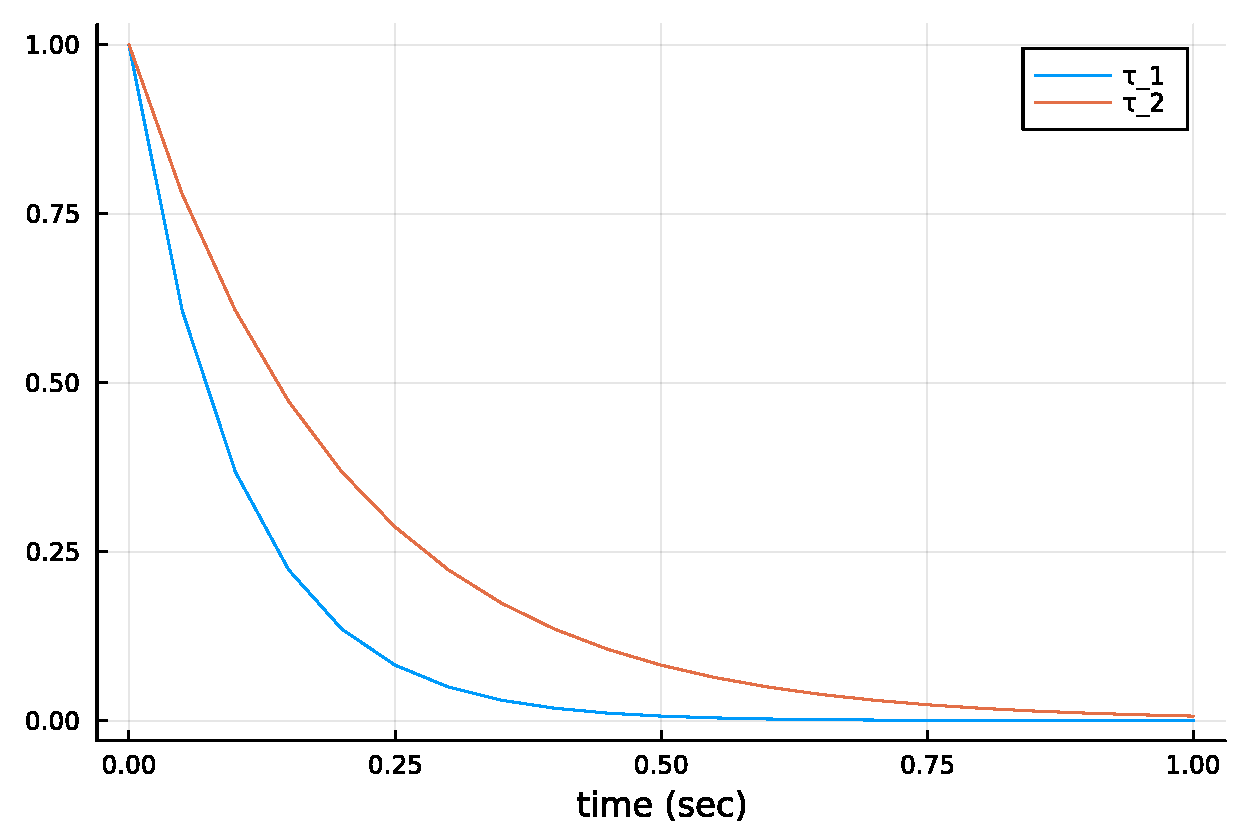
\includegraphics[width=4in]{diff_exp_decay}

\question Explain how two eigenmodes that independently exhibit exponential (geometric) decay can manifest in seemingly transient amplification in a different reference frame (e.g. a single neuron activity).
\vspace{\stretch{0.5}}

\subsection{Purely feedforward networks}
If there are no loops in the graph of the neural circuit, the neural activity of a neuron at time $t$ will never influence itself later (at least internally).
Let us call such neural circuits \textbf{purely feedforward}.

\question Consider a network of 3 neurons where neuron 1 excites neuron 2 and neuron 2 excites neuron 3? Draw the neural circuit graph.
What is the corresponding connectivity matrix?
\vspace{\stretch{0.5}}

\question Show that the connectivity matrix of any purely feedforward network can be written as a strictly triangular form (by choosing a certain ordering of neurons).
\vspace{\stretch{0.5}}


\subsection{Neural computation as filtering}
Given an input signal $x(t)$, a \textbf{filter} outputs a corresponding output signal $y(t)$ through a causal mechanism.
This captures the essence of biophysical computation at various scales--a transformation of a signal over time.
This transformation may also depend on the internal state of the neural system in general.

\subsection{Linear time invariant system}

\subsection{Finite impulse response}

\subsection{Rotated feedforward networks}


\subsection{Other cases}
Consider the following example permutation matrix:
\begin{align}\label{eq:nnm:ex:b}
W_b &=
\begin{bmatrix}
0 & 1 & 0\\
0 & 0 & 1\\
1 & 0 & 0
\end{bmatrix}
\end{align}


\section{Continuous-time Linear Dynamical Systems}
\subsection{Scope}
We want to study homogenuous differential equations with constant coefficients that can be written succintly in matrix form as
\begin{align}
    \dot{\vx}(t) &= F \vx(t)
\end{align}
\subsection{First order linear differential equations}
Consider the following first order homogenuous linear ODE with constant coefficients
\begin{align}
    &\dot{x}(t) + a x(t) = 0\\
    &x(0) = k
\end{align}
To solve the differential equation means to find the function $x(t)$ which passes through $c$ at time $t=0$ and has a derivative, which irregardless of time, is the function evaluation scaled by $a$.  Lets begin by making the formal rearrangement
\begin{align}
    &\frac{dx}{x} = - a \, dt\\
    \implies &x(t) = c_1 \exp(-at)
\end{align}
If we were not given the initial condition, $x(0)=k$, this is as far as we could go in determining a solution.  Fortunately, we can solve for $c_1$ by using the initial condition, so that $c_1 = k$.  Thus, the full solution to the differential equation is just $x(t) = k \exp(-at)$.  

\textbf{Remark}: The system this differential equation describes is not very interesting.  If $a < 0$ then $x(t) \rightarrow \infty$, whereas if $a > 0$ then $x(t) \rightarrow 0$.

\question {Draw the phase portrait for this first order system.}
\vspace{\stretch{0.5}}
\subsection{$N$-th order linear differential equations}
Lets consider a more interesting example where we consider the solution to an $N$-th order linear differential equation with constant coefficients given by
\begin{align}
    &\sum_{i=0}^N a_i x^{(i)}(t) = 0\\
    &x^{(i)}(0) = k_i \qquad i = 0, \ldots, N-1
\end{align}
% To solve this differential equation, we are going to make an \textit{ansatz}, i.e. we are going to assume the solution is of the form
% \begin{align}
%     x(t) = \exp(c t)
% \end{align}
% then of course, we have that
% \begin{align}
%     \dot{x}(t) &= c \exp(ct)\\
%     \ddot{x}(t) &= c^2 \exp(ct)
% \end{align}
% which would mean that
% \begin{align}
%     \exp(ct) \left(c^2 - c a_1 - a_2\right) = 0
% \end{align}
% Provided this ansatz is correct, we have to find $c$ such that $c^2 - ca_1 - a_2 = 0$, i.e. we have to find the roots of this polynomial.  Lets call the roots of this equation $c_1$ and $c_2$; there are three cases to examine: $i)$ when $c_1$ and $c_2$ are real and distinct roots, $ii)$ when $c_1$ and $c_2$ are complex conjugate, i.e. $c_1 = \alpha + j \beta$ and $c_2 = \alpha - j \beta$ and $iii)$ when $c_1 = c_2$.  

% Unfortunately, in the case of $iii)$, the ansatz is wrong.  At this point, most introductory material on differential equations will posit the existence of a solution of the form $x(t) = v(t) \exp(ct)$ and try to find what $v(t)$ should be.  However, we are going to stick with what we know -- and that is the solution of the first order homogenuous equation with constant coefficients.

% \section{Matrix form of an ODE}
without loss of generality $a_N = 1$.  If we define
\begin{align}
    \vx(t) &= \begin{bmatrix} x(t) & x^{(1)}(t) & \cdots & x^{(N-1)}\end{bmatrix}^\top
\end{align}
then we can transform this $N$-th order equation into a first order one below
\begin{align}\label{eq::matrixDifferential}
    &\dot{\vx}(t) = F \vx(t)\\
    &\vx(0) = \vk
\end{align}
by overloading the differential operator so that $\dot{\vx}(t) = \begin{bmatrix} x^{(1)}(t) & x^{(2)}(t) & \cdots & x^{(N)}\end{bmatrix}^\top
$, and setting
\begin{align}
    F = \begin{pmatrix} 0 & 1 & 0 & \cdots & 0 \\ 
                        0 & 0 & 1 & \cdots & 0 \\
                        \vdots & \vdots & \vdots & \ddots & \vdots\\
                        -a_1 & -a_2 & -a_3 & \cdots & -a_{N-1} \end{pmatrix}
\end{align}
\textbf{Remark}: A matrix in this form is said to be a companion form matrix.  They arise when we transform an $N$-th order differential equation into a first order system as we did above.

\subsection{Fundamental matrix solution}
How can we actually solve this matrix differential equation? That is, how can we find the vector that satisfies Eq.~\eqref{eq::matrixDifferential} and the associated initial condition? To answer this question, we have to take a slight detour and discuss the \textit{fundamental matrix solution}

Lets begin by assuming that we can find the solution to Eq.~\eqref{eq::matrixDifferential}, then if we denote the $N$ solutions as $\phi_1(t), \phi_2(t), \ldots, \phi_N(t)$ then we can write
\begin{align}
    &a_0 \phi_1(t) + a_1 \phi_1^{(1)}(t) + \cdots + \phi_1^{(N)}(t) = 0\\
    &a_0 \phi_2(t) + a_1 \phi_2^{(1)}(t) + \cdots + \phi_2^{(N)}(t) = 0\\
    & \qquad \qquad \qquad \qquad \vdots\\
    &a_0 \phi_N(t) + a_1 \phi_N^{(1)}(t) + \cdots + \phi_N^{(N)}(t) = 0
\end{align}
which if take $\Phi_i(t) = \begin{bmatrix} \phi_i(t) & \phi_i^{(1)}(t) & \cdots & \phi_i^{(N)}(t) \end{bmatrix}^\top$, and set 
\begin{align}
    \fundamentalSolution(t, 0) = \begin{pmatrix} \vline & \vline & & \vline\\
        \Phi_1(t) & \Phi_2(t) & \cdots & \Phi_N(t)\\
        \vline & \vline & & \vline
    \end{pmatrix}
\end{align}
then we can write that
\begin{align}
    \dot{\fundamentalSolution}(t, 0) = F \fundamentalSolution(t, 0)
\end{align}
Now, if we were to make an \textit{ansatz} and guess that the solution is $\vx(t) = \fundamentalSolution(t, 0) \vx(0)$ then we can easily verify whether or not this is true
\begin{align}
    &\dot{\vx}(t) = F \vx(t)\\
    \implies & \dot{\fundamentalSolution}(t, 0) \vx(0) = F \fundamentalSolution(t, 0) \vx(0)\\
    \implies & F \fundamentalSolution(t, 0) \vx(0) = F \fundamentalSolution(t, 0) \vx(0)
\end{align}
which also implies that $\fundamentalSolution(0, 0) = I$.  
\begin{tcolorbox}[colback=black!1!,title=Fundamental Solution]
    \begin{theorem}[Series representation of fundamental solution]
        The series of matrices, $M_0, M_1, M_2, \ldots$, defined recursively as
        \begin{align}
            &M_0 = I\\
            &M_k = I + F \int_0^t M_{k-1}(\sigma) d\sigma
        \end{align}
        converges uniformly to $\Phi(t, 0)$
    \end{theorem}
    If we expand the recursion above (which we could do with the aid of induction), we see something interesting
    \begin{align}
        \fundamentalSolution(t, 0) &= I + Ft + F^2 \frac{t^2}{2!} + F^3 \frac{t^3}{3!} + \cdots
    \end{align}
    If $F$ were a scalar, then this would exactly be the series representation of $\exp(Ft)$.  In fact, this infinite series is exactly how we define the \textit{matrix exponential}.
\end{tcolorbox}

\begin{tcolorbox}[colback=black!1!,title=Properties of the matrix exponential]
    \textbf{Diagonal matrices}: If $D = \diag(d_1, d_2, \ldots, d_N)$ then $\exp(D) = \diag(e^{d_1}, e^{d_2}, \ldots, e^{d_N} )$.\newline

    \textbf{Commuting matrices}: If $A$ and $B$ commute ($AB = BA$), then we have that $\exp(A + B) = \exp(A) \exp(B) = \exp(B) \exp(A)$.\newline

    \textbf{Inverse}: $\exp(A) \exp(-A) = I$
\end{tcolorbox}
\question {Prove the property about commuting matrices.}
\vspace{\stretch{0.5}}

In many cases $\fundamentalSolution(t, 0)$ is unwieldly to actually compute.  However, we are fortunate in that we are working with differential equations of constant coefficients; in this particular case, 
\begin{align}
    \fundamentalSolution(t, 0) = \exp(F t)
\end{align}
which we can verify satisfies both $\fundamentalSolution(0, 0) = I$ as well as
\begin{align}
    \frac{d}{dt} \exp(Ft) &= \frac{d}{dt} \left(I + Ft + F^2 \frac{t^2}{2!} + F^3 \frac{t^3}{3!}\cdots  \right)\\
    &= F + F^2 t + F^3 \frac{t^2}{2!} + \cdots\\
    &= F \exp(F t)
\end{align}
\subsection{Jordan form}
Since the matrix exponential is defined in terms of an infinite series, we are left wondering whether it can be computed analytically.  For this, we have to introduce the concept of a \textit{Jordan matrix}.  A matrix $J \in \reals^{M\times M}$ is said to be a Jordan matrix if it takes the form
\begin{align}
    J = \begin{pmatrix} \lambda & 1 & 0 & 0 & \cdots & 0\\
        0 & \lambda & 1 & 0 & \cdots & 0\\
        \vdots & \vdots & \vdots & \vdots & \ddots & \vdots\\
        0 & 0 & 0 & 0 & \cdots & \lambda
    \end{pmatrix}
\end{align}
which means we could write that $J = \lambda I + N$; this matrix $N$ is said to be nilpotent. 

\begin{tcolorbox}[colback=black!1!,title=Nilpotent matrices]
    A matrix $N$ is said to be nilpotent if there exists an integer $k$ such that $N^k = 0$
\end{tcolorbox}

\question Is the following matrix nilpotent? Support your claim either way.
\begin{align}
    Q = \begin{pmatrix} 0 & 1 & 0\\
    0 & 0 & 1\\
    0 & 0 & 0
\end{pmatrix}
\end{align}
\vspace{\stretch{0.5}}

% \question{Can you generalize this claim to general off diagonal matrices $N \in \reals^{M \times M}$.}
% \vspace{\stretch{0.5}}

As we have shown, $N$ and $\lambda I$ commute.  Combining the first two properties of the matrix exponential, this allows us to write that $    \exp(J t) = \exp(\lambda t) \exp(N t)$.  However, we still have more work to do as we have not yet computed $\exp(Nt)$.  Recalling that $N$ is nilpotent, we can write
\begin{align}
    \exp(Nt) &= \sum_{i=0}^{\infty} N^i \frac{t^i}{i!}\\
    &= \sum_{i=0}^{M-1} N^i \frac{t^i}{i!}\\
    &= \begin{pmatrix} 1 & t & \frac{t^2}{2!} & \frac{t^3}{3!} & \cdots & \frac{t^{M-1}}{(M-1)!}\\
        0 & 1 & t & \frac{t^2}{2!} & \cdots & \frac{t^{M-2}}{(M-2)!}\\
        \vdots & \vdots & \vdots & \vdots & \ddots & \vdots\\
        0 & 0 & 0 & 0 & \cdots & 1
    \end{pmatrix}
\end{align}
Great! Now we have the ability to easily calculate the matrix exponential of any Jordan form matrix.  Now we may ask, what about the matrix exponential of more general matrices? As it turns out, any matrix can be written in Jordan canonical form.
\begin{tcolorbox}[colback=black!1!,title=Jordan normal form]
    \textbf{Definition of Jordan Normal Form}: We say a matrix $J \in \reals^{N \times N}$ is in Jordan normal form if it can be written as follows:
    \begin{align}
        J = \begin{pmatrix} J_1 & 0 & \cdots & 0\\
        0 & J_2 & \cdots & 0\\
        0 & 0 & \cdots & J_K\end{pmatrix}
    \end{align}
    where each $J_i$ is a Jordan block matrix, i.e.
    \begin{align}
        J_i = \begin{pmatrix} \lambda_i & 1 & 0 & \cdots & 0\\
            0 & \lambda_i & 1 & \cdots & 0\\
            \vdots & \vdots & \vdots & \ddots & \vdots\\
            0 & 0 & 0 & \cdots & \lambda_i
        \end{pmatrix}
    \end{align}
\end{tcolorbox}

\subsection{Companion form matrices}
Consider an $N\text{-th}$ order polynomial of the form
\begin{align}
    p(x) = x^N + a_{N-1} x^{N-1} + \cdots + a_1 x + a_0
\end{align}
then, the matrix $F$ defined below is called a companion form matrix
\begin{align}
    F = \begin{pmatrix} 0 & 1 & 0 & \cdots & 0\\
                        0 & 0 & 1 & \cdots & 0\\
                        \vdots & \vdots & \vdots & \ddots & \vdots\\
                        -a_0 & -a_1 & -a_2 & \cdots & -a_{N-1}\end{pmatrix}
\end{align}
and we have that the eigenvalues of $F$ coincide with the roots of the characteristic polynomial defined by $p(x)$.  That is, if $\det(\lambda I - F) = 0$, then $p(\lambda) = 0$.  
\subsection{Linear differential equations}
We begin by examining $N-\text{th}$ order linear differential equations with constant coefficients
\begin{align}
    \dot{x}(t) &= A x(t)\\
    x(0) &= x_0
\end{align}
If $A$ is not in companion form, then we can always reason about the surrogate system
\begin{align}
    \dot{y}(t) &= F y(t)\\
    y(0) &= y_0
\end{align}
where $F$ is now a companion form matrix, that is similar to $A$.  The exact coordinate transformation can be found by taking the Jordan decomposition of $A$ and $F$
\begin{align}
    A &= T^{-1} J T\\
    F &= S^{-1} J S\\
\end{align}
then setting $x(t) = T^{-1} S y(t)$.
\subsection{Characteristic and minimal polynomials}
We define the characteristic polynomial 
\begin{align}
    p_{A}(x) = \det \left( x I - A \right)
\end{align}
and the minimal polynomial, $\chi_A(x)$, to be the lowest order polynomial which satisfies $\chi_A(A) = 0$.

\subsection{Functions of matrices}
\section{Nonlinear systems that are really linear}
\subsection{Linearization theorems}
Let us consider a (time-invariant and autonomous) nonlinear dynamical system:
\begin{align}
    \dot{x} = f(x)
\end{align}
where $x \in \reals^n$ and $f: \reals^n \to \reals^n$.
Much of this nonlinear dynamical system can be understood piece by piece using our knowledge of linear dynamical systems.

\begin{tcolorbox}[colback=black!1!,title=Linearize that beast!]
    Most nonlinear dynamical systems are locally a linear dynamical system, but strange non-local things can happen.
\end{tcolorbox}

In particular, the dynamics around equilibria (fixed points) are topologically conjugate to that of the linearization.
Let $\bar{x}$ be a fixed point of the dynamics that is, $f(\bar{x}) = 0$.
Note that there are potentially many or infinitely many fixed points.
Let $[Df]_{i,j}(\bar{x}) = \frac{\partial f_i}{\partial x_j}\bigr\rvert_{\bar{x}}$ be the Jacobian (matrix), i.e., linearization of the dynamics at $\bar{x}$:
\begin{align}\label{eq:linearized_around_FP}
    \dot{x} = Df(\bar{x}) (x - \bar{x})
\end{align}


\begin{theorem}[Hartman-Grobman]
    If $Df(\bar{x})$ has no zero or purely imaginary eigenvalues then there is a homeomorphism $h$ defined on some neighborhood $U$ of $\bar{x}$ in $\reals^n$ locally taking obits of the nonlinear flow $\phi_t$ to those of the linear flow.
\end{theorem}
As the theorem states, linearlization around the fixed point fails if there are eigenvalues with zero real part.
They are typically rare in practice, but of great interest to nonlinear dynamics analysis and important for bifurcation theory.
Fixed points that allows linearlization are called \textbf{hyperbolic} fixed points.
For hyperbolic fixed points, the stability of nonlinear system is equivalent to that of the linearized system.

Away from the fixed points, the flow of nonlinear dynamical system is topologically conujugate to a boring constant flow:
\begin{theorem}[Rectification]
    If $p \in \reals^n$ and $f(p) \neq 0$, then there are open sets $U, V \in \reals^n$ with $p \in U$ and a diffiomorphism $g: U \to V$ such that the differential equation in the new coordinates, that is, the differential equation,
    $$ \dot{y} = Dg(g\inv(y)) f(g\inv(y)), $$
is given by $(\dot{y}_1, \ldots, \dot{y}_n) = (1, 0, 0, \ldots, 0)$.
\end{theorem}
See \citet[Lemma 1.120]{Chicone2006}.

Of course, a patchwork of linear dynamics can create some interesting systems.
In neural data analysis, locally linear dynamical system model~\cite{Zhao2016d} and recurrent switching linear dynamical systems type models utilize this~\citep{Linderman2017,Nassar2018b}.

\begin{align}\label{eq:cubicode}
\begin{split}
\dot x &= x^3 + y\\
\dot y &= 3x \\
\end{split}
\end{align}

\begin{figure}[h]
    \centering
    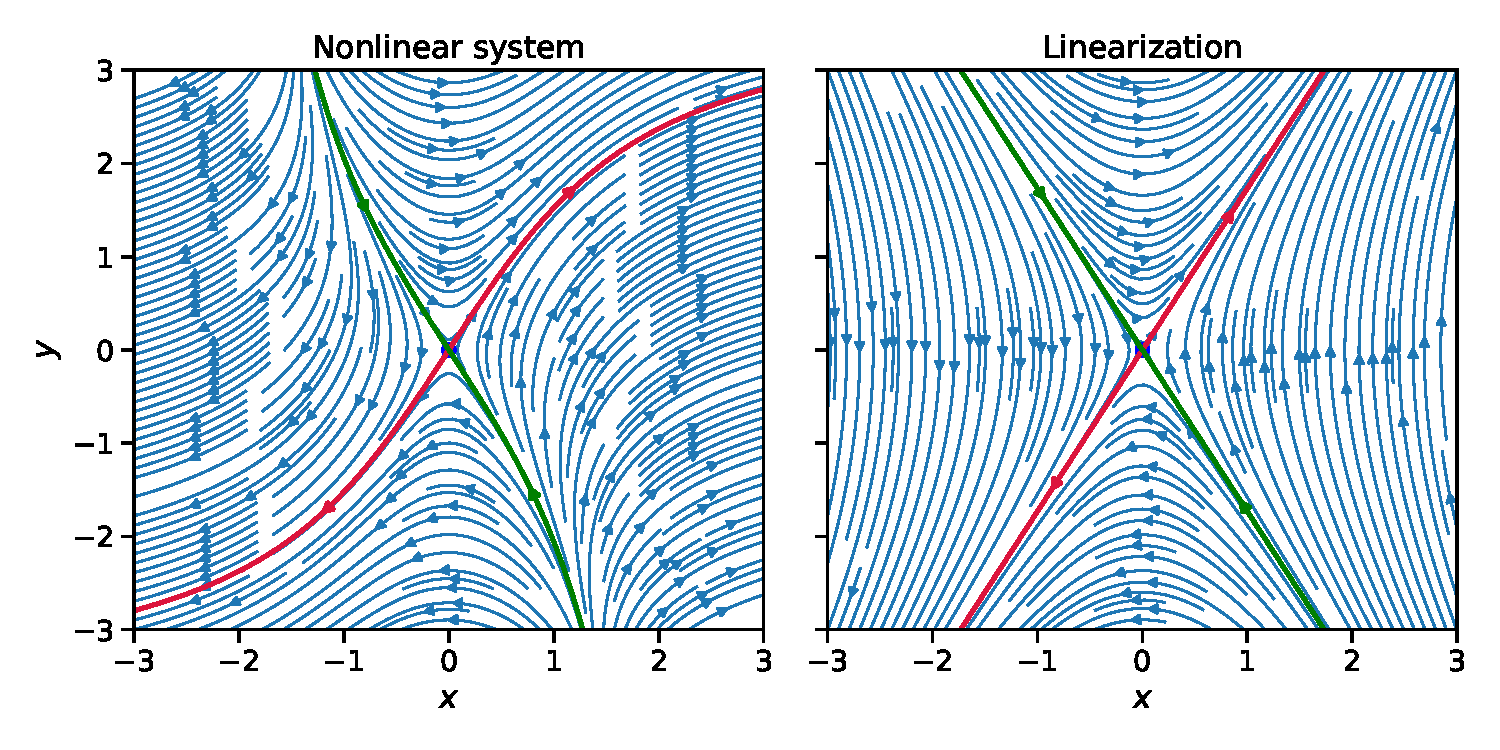
\includegraphics[width=\textwidth]{linearization}
    \caption{Linearization of the system described in Equation \ref{eq:cubicode}.}
    \label{fig:linearization}
\end{figure}

\subsection{Kernel methods}
When linear methods fail due to nonlinearity, you can always try linear methods applied to a nonlinearly mapped space.

All you need is an inner product to implement many linear methods (least squares regression, PCA, CCA, k-means).

\begin{tcolorbox}[colback=black!1!,title=Kernel Trick]
You can implicitly map your data to an infinitely high-dimensional space by using a (positive semi-definite) \textbf{kernel}.
\end{tcolorbox}

\subsection{Koopman operators}

\end{questions}

\section*{Acknowledgements}
Special thanks to Ayesha Vermani and \'Abel S\'agodi.

\bibliographystyle{plainnat}
\bibliography{refs}
\end{document}
